% Seção de Metodologia
\section{Revisão da Literatura}
% Slide da seção de Metodologia

%%
%%
%%
% \begin{frame}{Revisão Sistemática}
%     % Formulação da Revisão Termos Chave
%     % 3 colunas: Termos Chave | Criterios de Inclusão Exclusão | Snowballing

%     \begin{footnotesize}
        
%     \begin{minipage}[t]{0.26\textwidth}
%     \textbf{Termos Chave}
%     \begin{itemize}
%         \item Médico
%         \item Alocação
%         \item Programação Inteira
%         \item Otimização
%     \end{itemize}
%     \end{minipage}
%     \hfill
%     \begin{minipage}[t]{0.33\textwidth}
%     \textbf{Critérios de Inclusão}
%     \begin{itemize}
%         \item Focos em alocação médica no contexto clínico
%         \item Apresenta técnicas de otimização como forma de solução 
%     \end{itemize}

%     \textbf{Critérios de Exclusão}
%     \begin{itemize}
%         \item Contexto não clínico ou hospitalar
%         \item Não foca na força de trabalho médica
%         \item Não foca em métodos de Otimização
%     \end{itemize}
%     \end{minipage}
%     \hfill
%     \begin{minipage}[t]{0.3\textwidth}
%     \textbf{Snowballing}
%     \begin{itemize}
%         \item \citeonline{Abdalkareem_Amir_Al_Betar_Ekhan_Hammouri_2021}
%         \item \citeonline{Erhard_Schoenfelder_Fügener_Brunner_2018}
%         \item \citeonline{Ngoo_Goh_Sze_Sabar_Abdullah_Kendall_2022}
%     \end{itemize}
%     \end{minipage}

%     \end{footnotesize}

% \end{frame}

%
%
%

\begin{frame}{Revisão Sistemática}
    \begin{figure}
        \centering
        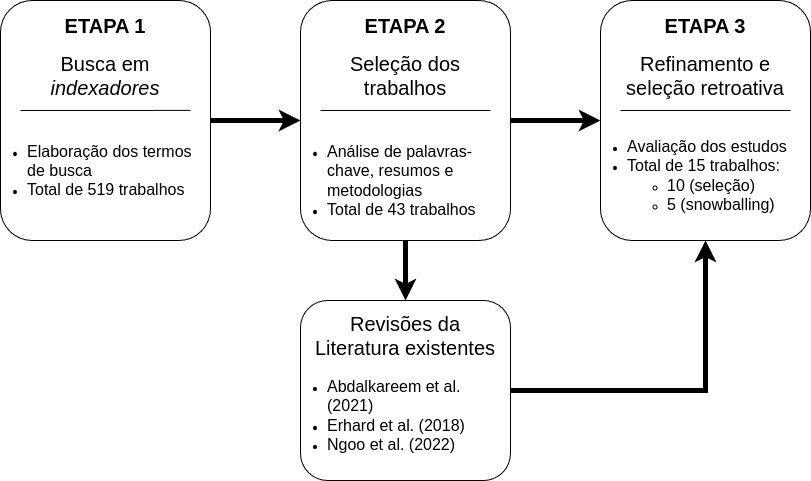
\includegraphics[width=0.95\linewidth]{img/rev-sist-quali.png}
        \caption{Processos da revisão realizada durante o estudo.}
        \label{fig:enter-label}
    \end{figure}
\end{frame}

%%
%%
%%
\begin{frame}{Trabalhos Similares}
    % Aqui vem a tabela de trabalhos
    \begin{figure}
        \centering
        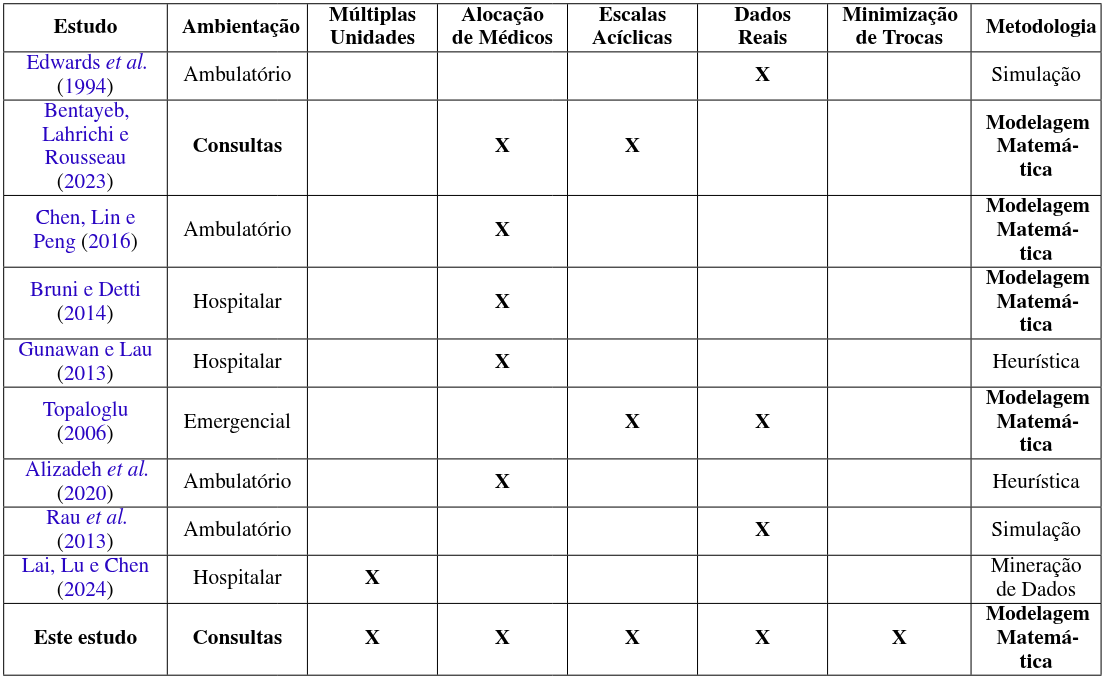
\includegraphics[width=0.9\linewidth]{img/trabalhos-correlatos.png}
        \caption{Trabalhos similares obtidos e avaliados}
        % \footnotesize{Fonte: Elaborado pelo autor.}
        \label{fig:enter-label}
    \end{figure}
    
\end{frame}

%%
%%
%%
\begin{frame}{Lacunas de Pesquisa}
    % Lacunas que este trabalho ataca
    \begin{block}{Este trabalho foca portanto...}
        \begin{itemize}
            \item Escalonamento Médico
            \item Contexto clínico
            \item Múltiplas Unidades simultaneamente
            \item Dados Reais
            \item Minimização de Trocas/Minimização de exames não atendidos.
        \end{itemize}
    \end{block}
\end{frame}

